
\hypertarget{wikidata-and-the-cell-ontology-interplay}{%
\subsection{Wikidata and the Cell Ontology interplay}\label{wikidata-and-the-cell-ontology-interplay}}

The contributions to cell types on Wikidata will be of most value if they are integrated to the current state-of-art of knowledge representation.
Arguably, the Cell Ontology is the main source of cell type identifiers in the context of the Human Cell Atlas project.{[}\protect\hyperlink{ref-qT8WxqjA}{42}{]}
Thus, data about cell types on Wikidata must be connected to the Cell Ontology.

To start the improvement in the interplay of both databases, we proposed and got the approval of a specific Wikidata identifier for the Cell Ontology, the ``Cell Ontology ID'' (\url{https://www.wikidata.org/wiki/Property:P7963}).
IDs can be added to Wikidata entities and connected them to external databases enabling integrative SPARQL queries.
Besides using the common Wikidata interface, one can crowd-curate identifiers via a 3rd-party service, Mix'N'Match, which provides a user-friendly framework for connecting identifier catalogues to Wikidata. {[}\protect\hyperlink{ref-JgiKEEdq}{155}/?p=114{]}, as seen in Figure \ref{fig:mixn_match_cl}.
Logically, we created a Mix'N'Match catalogue for harmonizing Cell Ontology IDs to Wikidata (\url{https://mix-n-match.toolforge.org/\#/catalog/4719}), harnessing the community support for the task.

\begin{figure}
\hypertarget{fig:mixnmatch_cl}{%
\centering
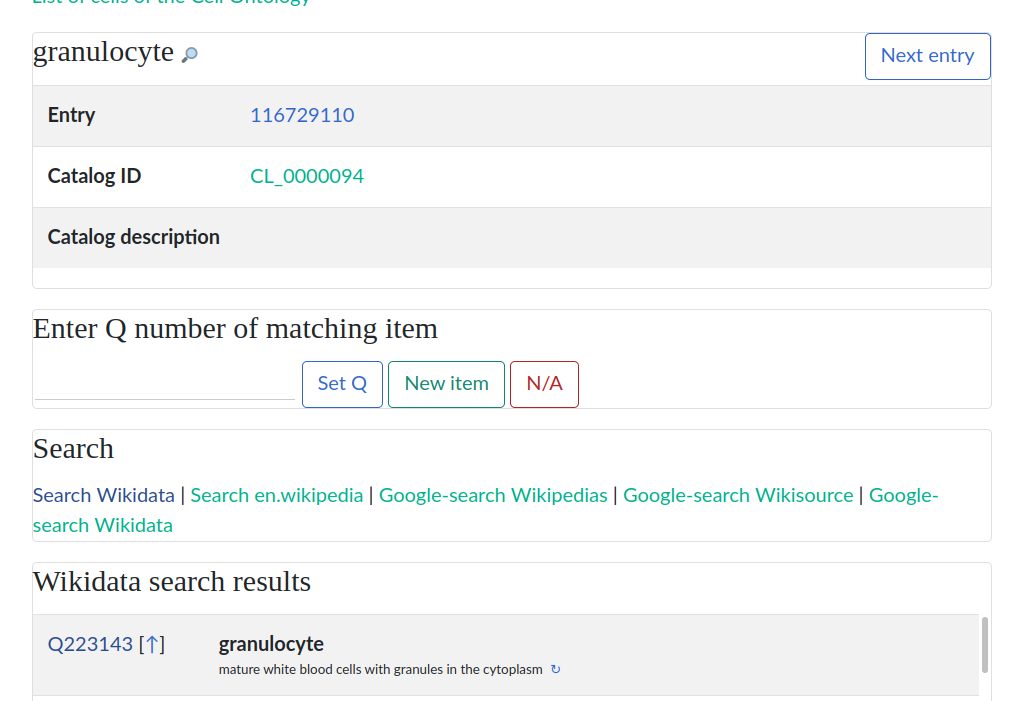
\includegraphics[width=0.85\textwidth,height=\textheight]{images/image-17.png}
\caption{Mix'N'Match curation system}\label{fig:mixnmatch_cl}
}
\end{figure}
